\capitulo{4}{Técnicas y herramientas} \label{chapter:tecnicas}

En este capítulo, se recogen las tecnologías principales empleadas en el desarrollo del proyecto, así como los detalles más relevantes de su implementación.

Para facilitar la organización y comprensión de las mismas, se han separado en tres subsecciones: \hyperref[sec:model]{Modelo}, \hyperref[sec:backend]{\emph{Backend}} y \hyperref[sec:frontend]{\emph{Frontend}}.


\section{Modelo} \label{sec:model}

Como se ha venido mencionando a lo largo de los anteriores capítulos, nuestro proyecto, a la hora de generar resúmenes, solo hace uso del modelo T5 de Google \cite{raffel19} por el momento. Más concretamente, utilizamos la implementación \texttt{t5-large} Hugging Face \cite{t5-hf}, el cual ha sido entrenado con texto en inglés, procedente del Colossal Clean Crawled Corpus (C4), y contiene aproximadamente 770 millones de parámetros \cite{hf-pretrained}.

Esta implementación está escrita en Python, lo que nos facilita la integración con el resto de componentes de JIZT, también desarrollados en Python.

El modelo \texttt{t5-large} consta, por un lado, del \emph{tokenizer}, encargado de la codificación del texto, y por otro, el modelo en sí, el cual recibe el texto codificado por el \emph{tokenizer}, y genera el resumen a partir de él. Dicho resumen, sigue estando en forma de \emph{tókenes} codificados, por lo que tenemos que hacer uso una vez más del \emph{tokenizer} para proceder a su decodificación. Una vez decodificado, el texto vuelve a contener caracteres legibles.

Tanto el proceso de codificación, como el de generación de resúmenes, se pueden llevar a cabo empleando unidades de procesamiento gráfico (GPU). No obstante, en nuestro caso, ambos procesos se ejecutan en unidades centrales de procesamiento (CPU), debido a limitaciones económicas\footnote{Cabe recordar que los modelos se ejecutan en <<la nube>>. Contratar equipos que dispongan de GPU aumentaría notablemente los costes.}. Esto explica en parte los \hyperref[table:comparativa]{tiempos de resumen obtenidos}.

Un último aspecto a destacar es que a la hora de generar los resúmenes, se pueden especificar los parámetros concretos con los que realizar dicha generación, permitiéndonos hacer uso de las diferentes estrategias vistas en la \autoref{subsec:estrategias-gen}.

\section{\emph{Backend}} \label{sec:backend}

En la \autoref{fig:overview-arch} se recoge una visión general de la arquitectura que conforma el \emph{backend} de JIZT, y que posibilita la implementación en la nube de las diferentes etapas en la generación de resúmenes descritas en el capítulo de \hyperref[chapter:conceptos]{Conceptos teóricos}.

\begin{figure}[!h]
	\centering
	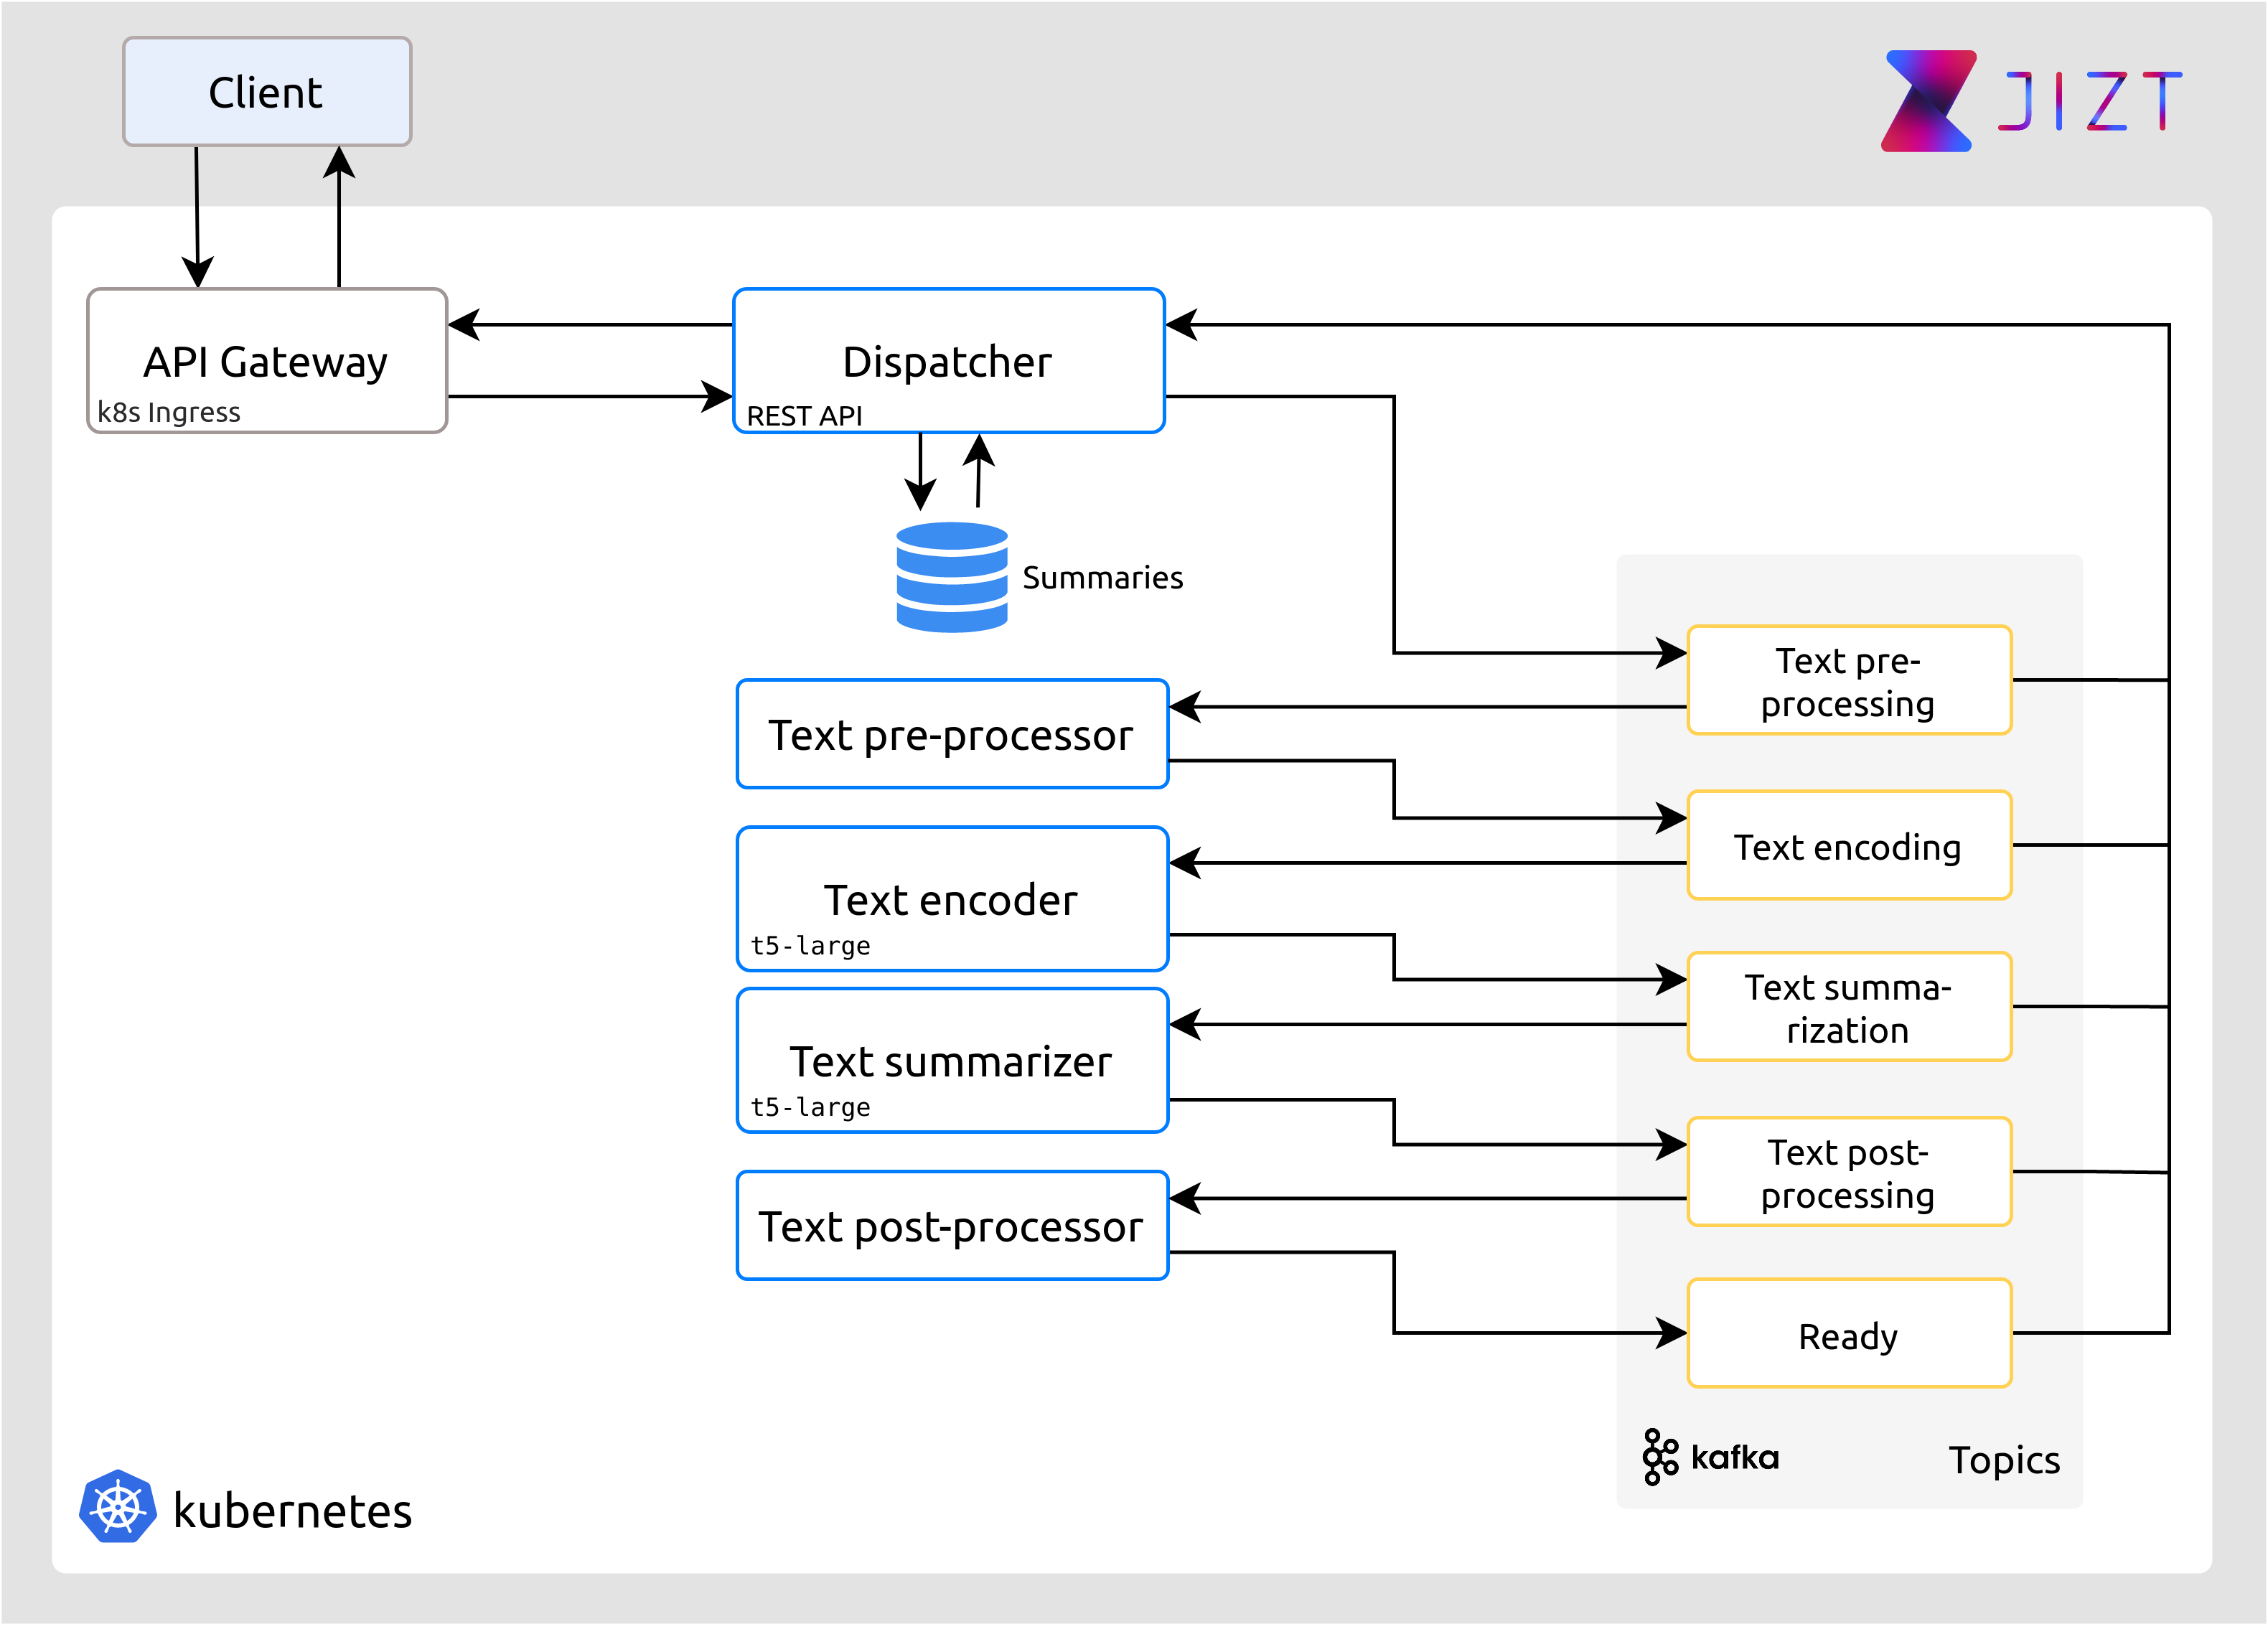
\includegraphics[width=\textwidth]{overview-arch}
	\caption{Vista general de la arquitectura del \emph{backend}.}
	\label{fig:overview-arch}
\end{figure}

En esta arquitectura, existen diferentes tecnologías, cada una encargada de realizar una tarea específica, pero a su vez integrándose con el resto. Veamos con más detalle cuáles son las características principales de dichas tecnologías.

\subsection{Kubernetes}

El \emph{backend} sigue una arquitectura de microservicios \cite{newman15}, de forma que cada una de las etapas (pre-procesado, codificación, generación del resúmen y post-procesado), está confinada en un contenedor Docker \cite{docker}, conformando un microservicio. Adicionalmente, existe un microservicio más, el \emph{Dispatcher}, el cual lleva a cabo las siguientes tareas:

\vspace{-0.5cm}
\begin{itemize}
	\item [\textbullet] Implementa una API REST que permite a los clientes solicitar resúmenes.
	\item [\textbullet] Gestiona una base de datos en la que se almacenan los resúmenes generados.
	\item [\textbullet] Redirige las peticiones de los clientes al microservicio apropiado. Por ahora, todas las peticiones se redirigen hacia el pre-procesador de textos, pero en un futuro podría existir otro microservicio que se encargara, por ejemplo, de extraer el texto de un documento PDF o de una página \emph{web}. En estos casos, el \emph{Dispatcher} se encargaría de redirigirlo hacia el microservicio correspondiente.
\end{itemize}

Kubernetes es una plataforma \emph{open-source} destinada a la gestión de servicios y cargas de trabajo en contenedores, que facilita su automatización en cuanto a aspectos como el escalado, gestión de red y recursos, monitorización, etc. \cite{kubernetes}

Kubernetes comprende numerosos componentes, entre los cuales, los más relevantes en nuestro caso son:

\vspace{-0.5cm}
\begin{itemize}
	\item [\textbullet] \emph{Pod}: es la unidad de computación básica en Kubernetes. Un \emph{Pod} puede ejecutar uno o varios contenedores intrínsecamente relacionados (compartirán almacenamiento, red, recursos, etc.). 
	\item [\textbullet] \emph{Deployment}: los \emph{deployments} se pueden ver como <<plantillas>> o <<moldes>> que contienen los detalles específicos para crear \emph{pods} de un determinado tipo. Por ejemplo, en el caso del mencionado \emph{Dispatcher}, dispondremos de un \emph{deployment} que indicará cómo se deben crear los \emph{pods} para este servicio. Estos \emph{pods} a su vez, contendrán todos la misma imagen Docker que implementará la lógica del servicio.
	\item [\textbullet] \emph{Service}: cada \emph{pod} dispone de una dirección IP propia. Sin embargo, los \emph{pods} tienen un ciclo de vida \emph{efímero}, dado que están concebidos para ser reemplazados dinámicamente si se producen errores, actualizaciones, etc. Por tanto, no podemos basar la configuración de red en las IPs específicas de los \emph{pods}, ya que estás son susceptibles de cambiar a lo largo del tiempo, según los \emph{pods} vayan siendo reemplazados. Los \emph{services} nos permiten asociar una IP fija y persistente a un conjunto concreto de \emph{pods}. A la hora de realizar una conexión con dicha IP, Kubernetes se encarga de remitir los datos al \emph{pod} que esté menos ocupado en ese instante, realizando por tanto un balance de carga de forma automática.
	
	\item [\textbullet] \emph{PersistentVolume}: al igual que en el caso de las IPs, los datos almacenados localmente en un \emph{pod} desaparecerán cuando este sea reemplazado. Los \emph{PersistentVolumes} nos proporcionan la capacidad de almacenar datos de manera persistente, independientemente del ciclo de vida de los \emph{pods}. Nosotros, utilizamos este componente para almacenar los modelos de generación de resúmenes, ya que ocupan alrededor de 5 GB, de forma que los \emph{pods} correspondientes a la codificación de texto y generación de resumen consumen los modelos desde una única fuente de datos, el \emph{PersistentVolume}. Incluir los modelos dentro de los propios \emph{pods} sería contraproducente porque (a) todos los \emph{pods} van a hacer uso de los mismos modelos, y (b) los modelos ocupan alrededor de los 5 GB, por lo que si quisiéramos crear varios \emph{pods}, la demanda de almacenamiento crecería rápida e innecesariamente.
\end{itemize}

La \autoref{fig:k8s-components} pretende facilitar la comprensión de los diferentes componentes de manera más visual. Como podemos ver en dicha figura, existen \emph{n} \emph{pods}, todos ellos replicas de un mismo \emph{deployment} y, por tanto, ejecutando los mismos contenedores, pero cada uno de ellos con una dirección IP propia. El \emph{service} permite acceder a los diferentes \emph{pods} a través de una única IP estática. Por último, todos los \emph{pods} consumen un mismo \emph{PersistentVolume} que, por ejemplo, podría contener los modelos ya mencionados.

\begin{figure}[!h]
	\centering
	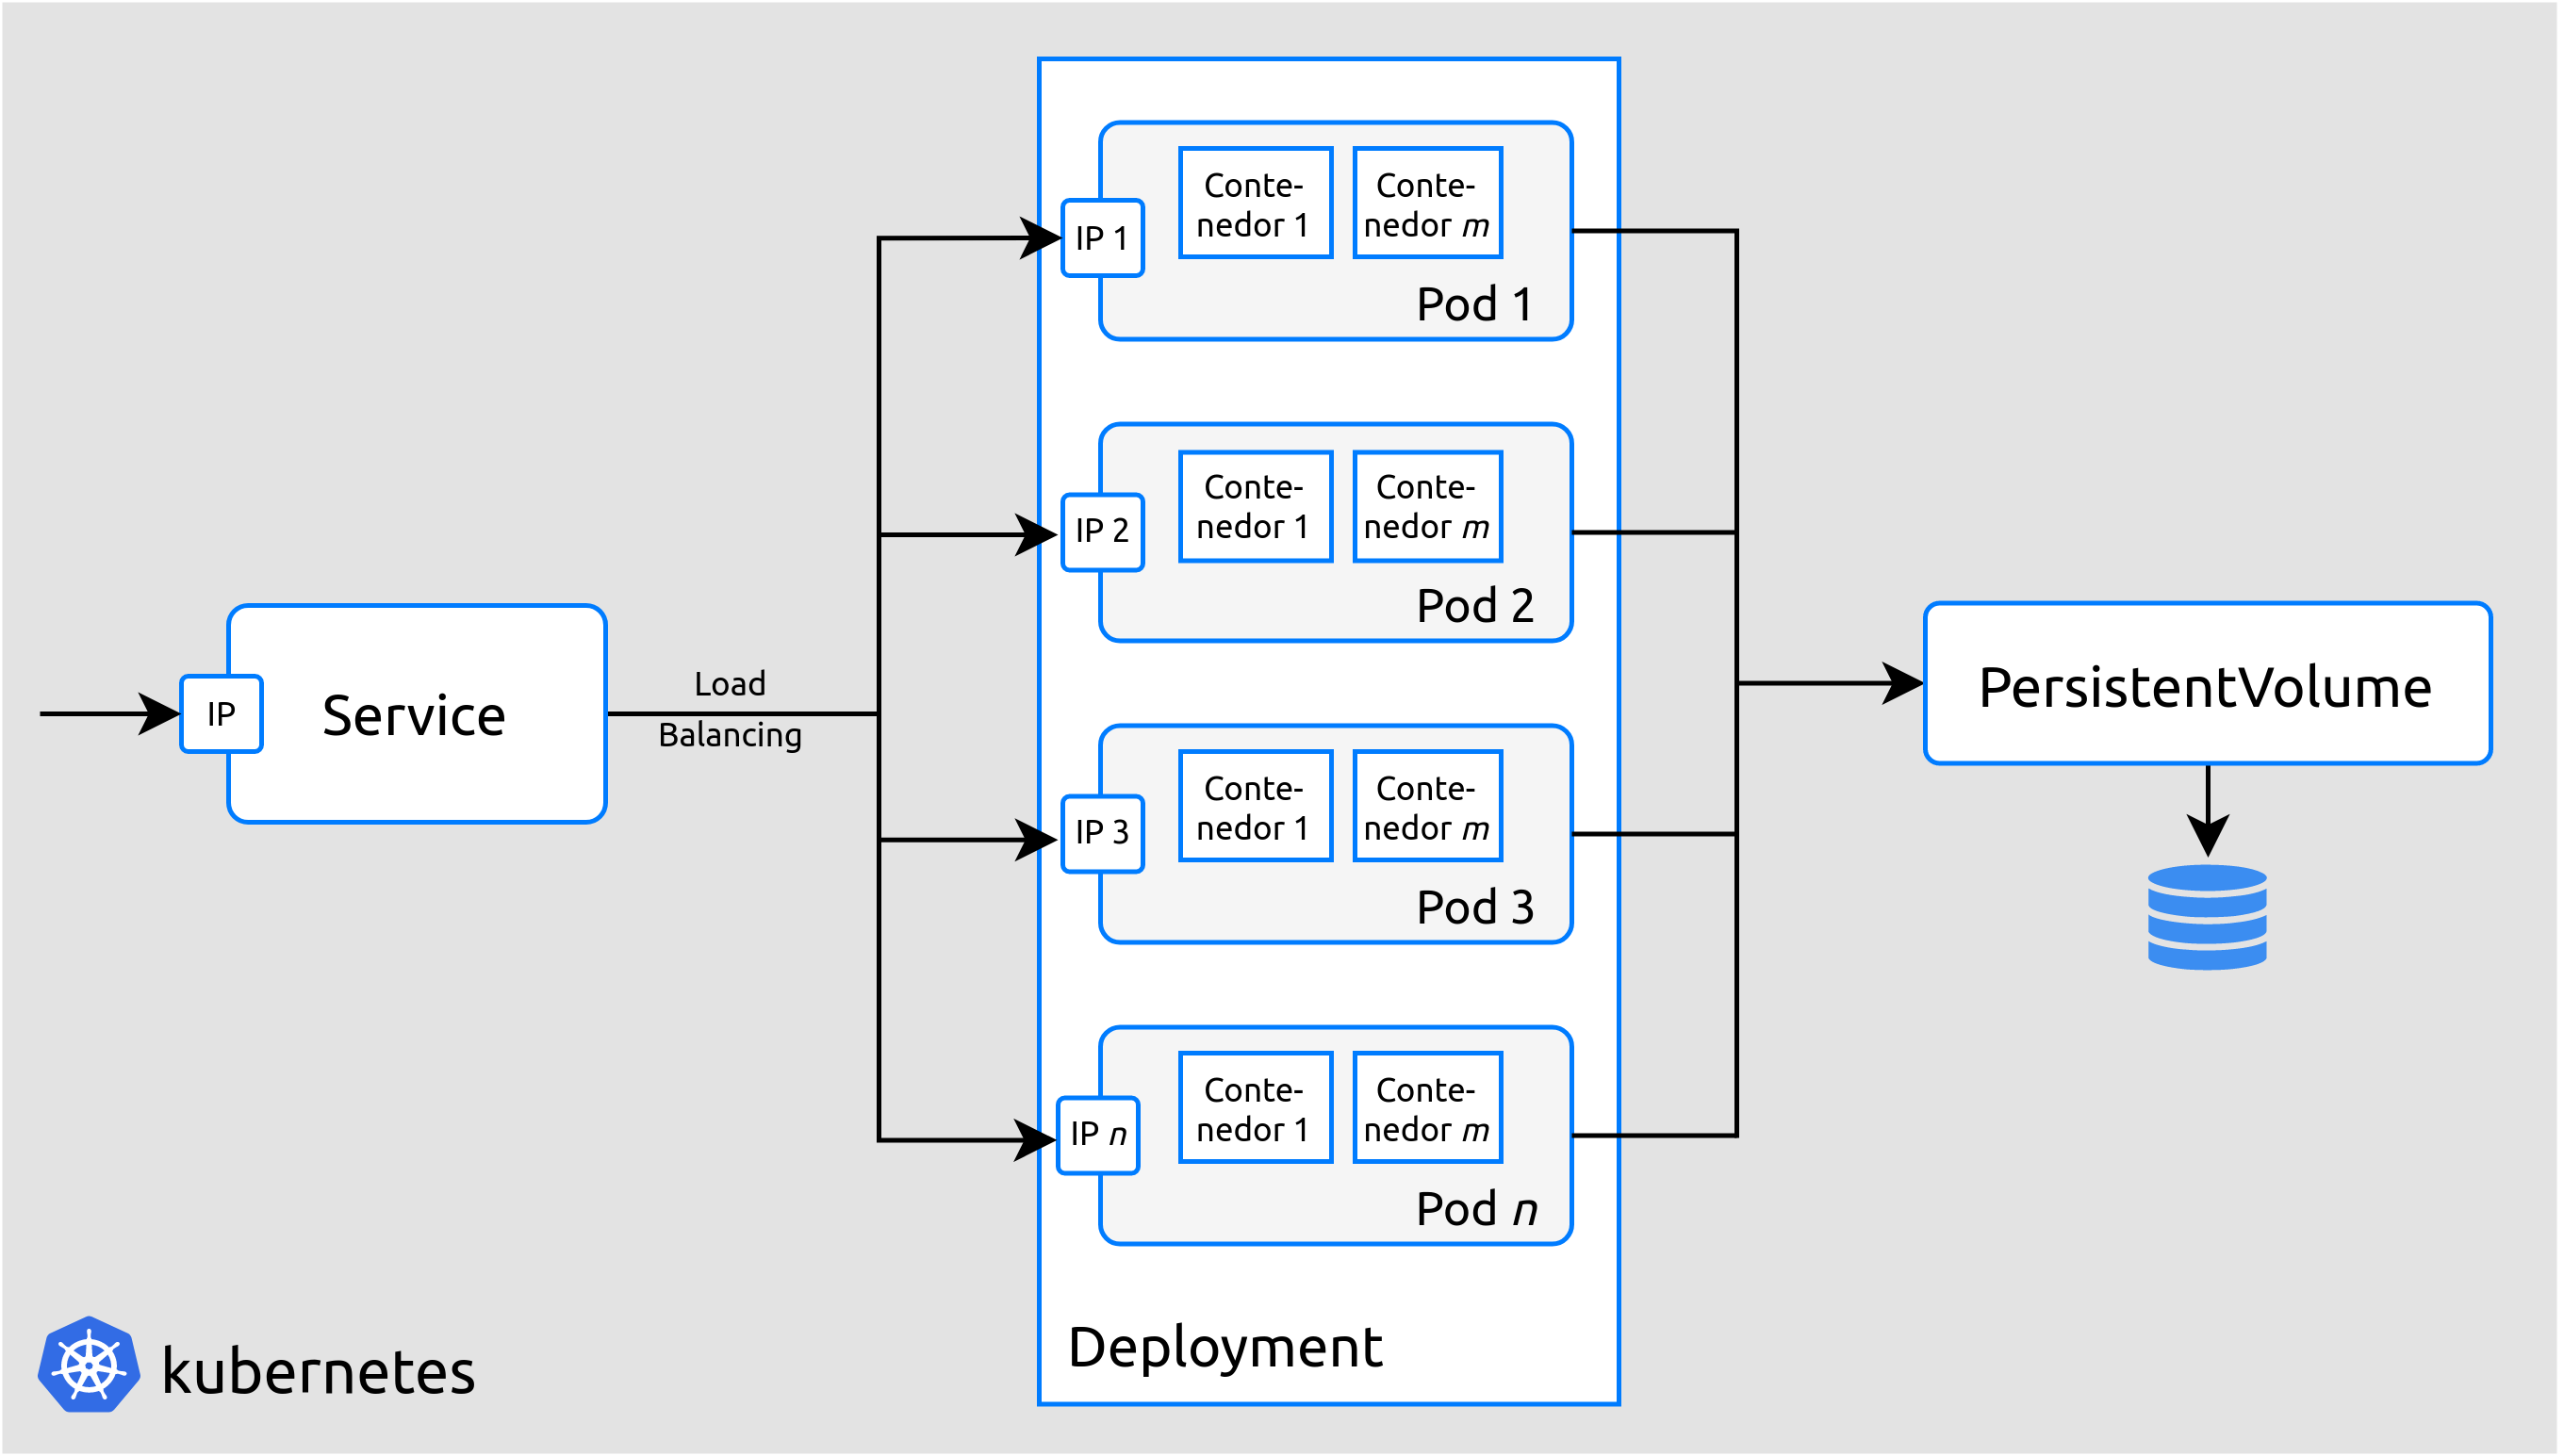
\includegraphics[width=\textwidth]{kubernetes-components}
	\caption{Componentes principales de Kubernetes.}
	\label{fig:k8s-components}
\end{figure}

De este modo, podemos escalar (o actualizar) cada uno de los microservicios de forma dinámica y sin periodos de inactividad (\emph{downtime}). De hecho, Kubernetes permite configurar el escalado de manera automática. Así, en momentos en los que la carga de trabajo sea mayor, se crearán \emph{pods} adicionales para responder ante dicha carga y, una vez esta desaparece, se volverán a eliminar. Al habilitar esta opción, es muy recomendable configurar el número máximo de \emph{pods} que se podrán creer, a fin de evitar un escalado descontrolado en momentos de carga extrema (en cualquier caso, Kubernetes detendría la creación de \emph{pods} tan pronto como se consumieran los recursos del sistema disponibles \cite{k8s-scheduling}).

Existe un último componente de Kubernetes del que hacemos uso, llamado Ingress. Este componente implementa una API \emph{Gateway}, enrutando las peticiones API de los clientes hacia el microservicio correspondiente \cite{api-gateway}. Por ahora, la API REST que hemos implementado solo dispone de rutas relacionadas a la generación de resúmenes, pero en un futuro, cuando se implementen otras tareas de NLP, existirán otros \emph{endpoints} para dichas tareas. Ingress se encargará entonces de, en función de a qué \emph{endpoint} se esté realizando la petición, redirigirla al microservicio correspondiente.

\begin{figure}[!h]
	\centering
	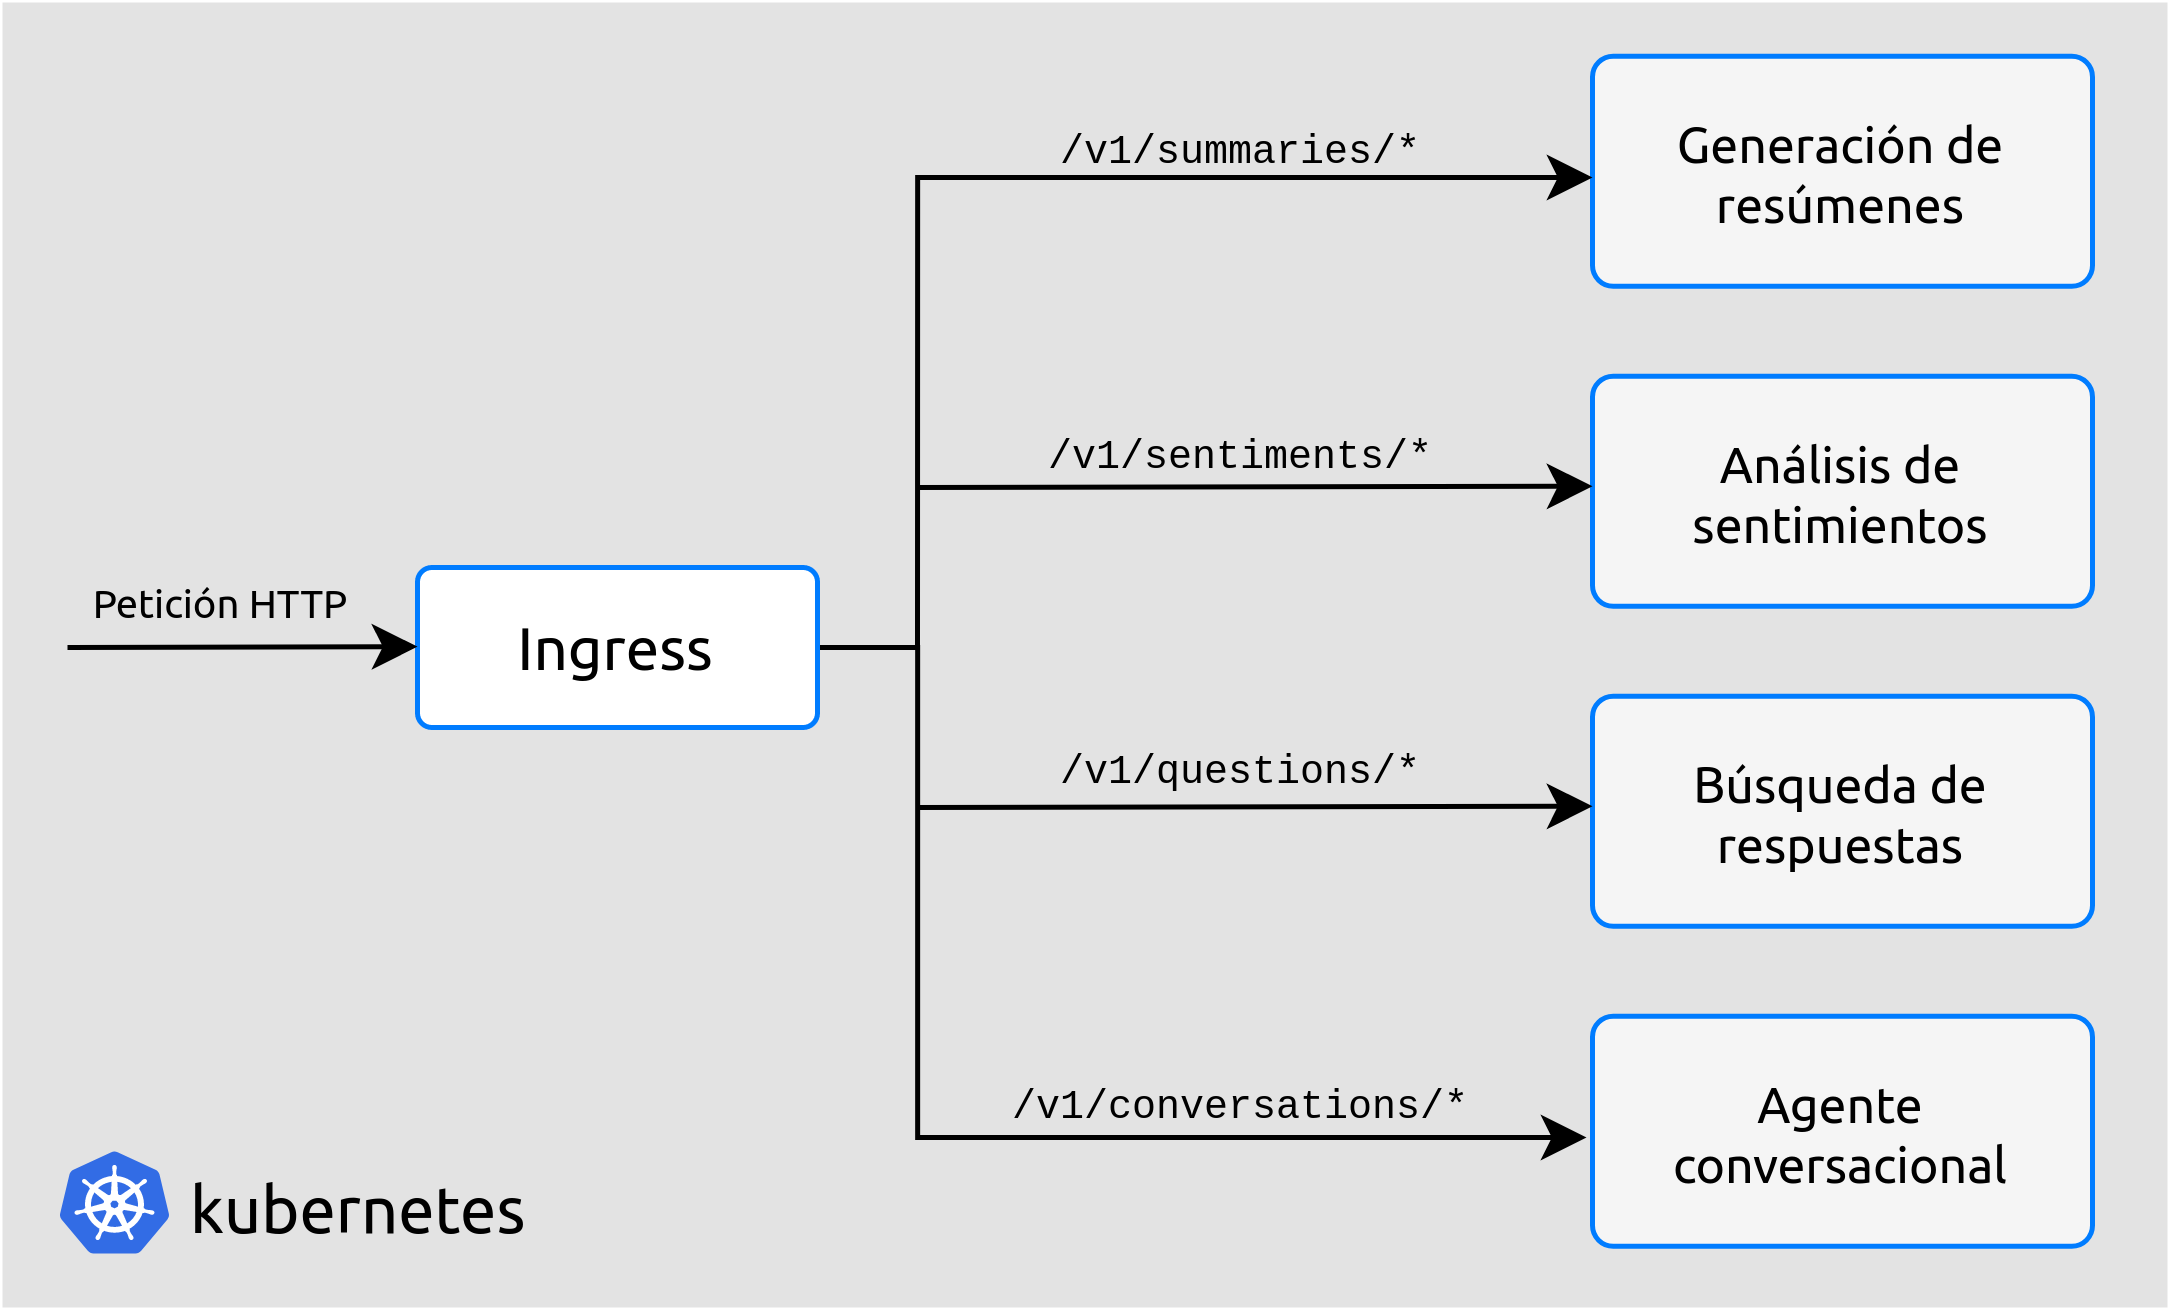
\includegraphics[width=0.9\textwidth]{kubernetes-ingress}
	\caption{Ejemplo de uso de Ingress con diferentes rutas.}
	\label{fig:k8s-ingress}
\end{figure}


\subsection{Kafka y Strimzi} \label{subsec:kafka}

Uno de los principales aspectos a considerar a la hora de implementar una arquitectura de microservicios reside en la estrategia que se va seguir para permitir la comunicación entre los diferentes microservicios.

Dicha comunicación puede llevarse a cabo de forma síncrona, por ejemplo a través de peticiones HTTP, o asíncrona, con tecnologías como Apache Kafka \cite{microsoft-microsvcs}.

En nuestro caso la comunicación síncrona quedó rápidamente descartada, dado que la generación de resúmenes presenta tiempos de latencia que pueden ser elevados (del orden de segundos o incluso minutos).

Apache Kafka nació internamente en LinkedIn, aunque actualmente es \emph{open-source} y su desarrollo corre a cargo de la Apache Software Foundation \cite{wiki-kafka}.

Kafka permite el intercambio asíncrono de mensajes entre productores y consumidores. En esencia, su funcionamiento es conceptualmente sencillo y está alineado con tecnologías más tradicionales: los consumidores se subscriben a un tema (\emph{topic}), a los que los productores envían sus mensajes. La consumición de dichos mensajes es asíncrona.

La novedad de Kafka reside entre otras cosas, en su gran capacidad de escalado, soportando billones de mensajes al día; su funcionamiento distribuido, permitiendo fácilmente operar a lo largo de diferentes zonas geográficas; su gran fiabilidad en entornos críticos, en los que la pérdida de un solo mensaje es inadmisible; o su tolerancia frente a fallos \cite{apache-kafka}.

Todas estas demandas no suponen, sin embargo, que Kafka no se pueda aplicar de igual modo a entornos más reducidos, como es el nuestro. Además, gracias a Strimzi, otro proyecto también \emph{open-source}, el despliegue de Kafka en Kubernetes se simplifica en gran medida.

Si volvemos a observar la \hyperref[fig:overview-arch-2]{figura} que incluíamos al principio de esta sección, podemos ver que JIZT dispone de cinco \emph{topics}, los cuales se corresponden con cada una de las etapas en la generación resúmenes:

\begin{figure}[!h]
	\centering
	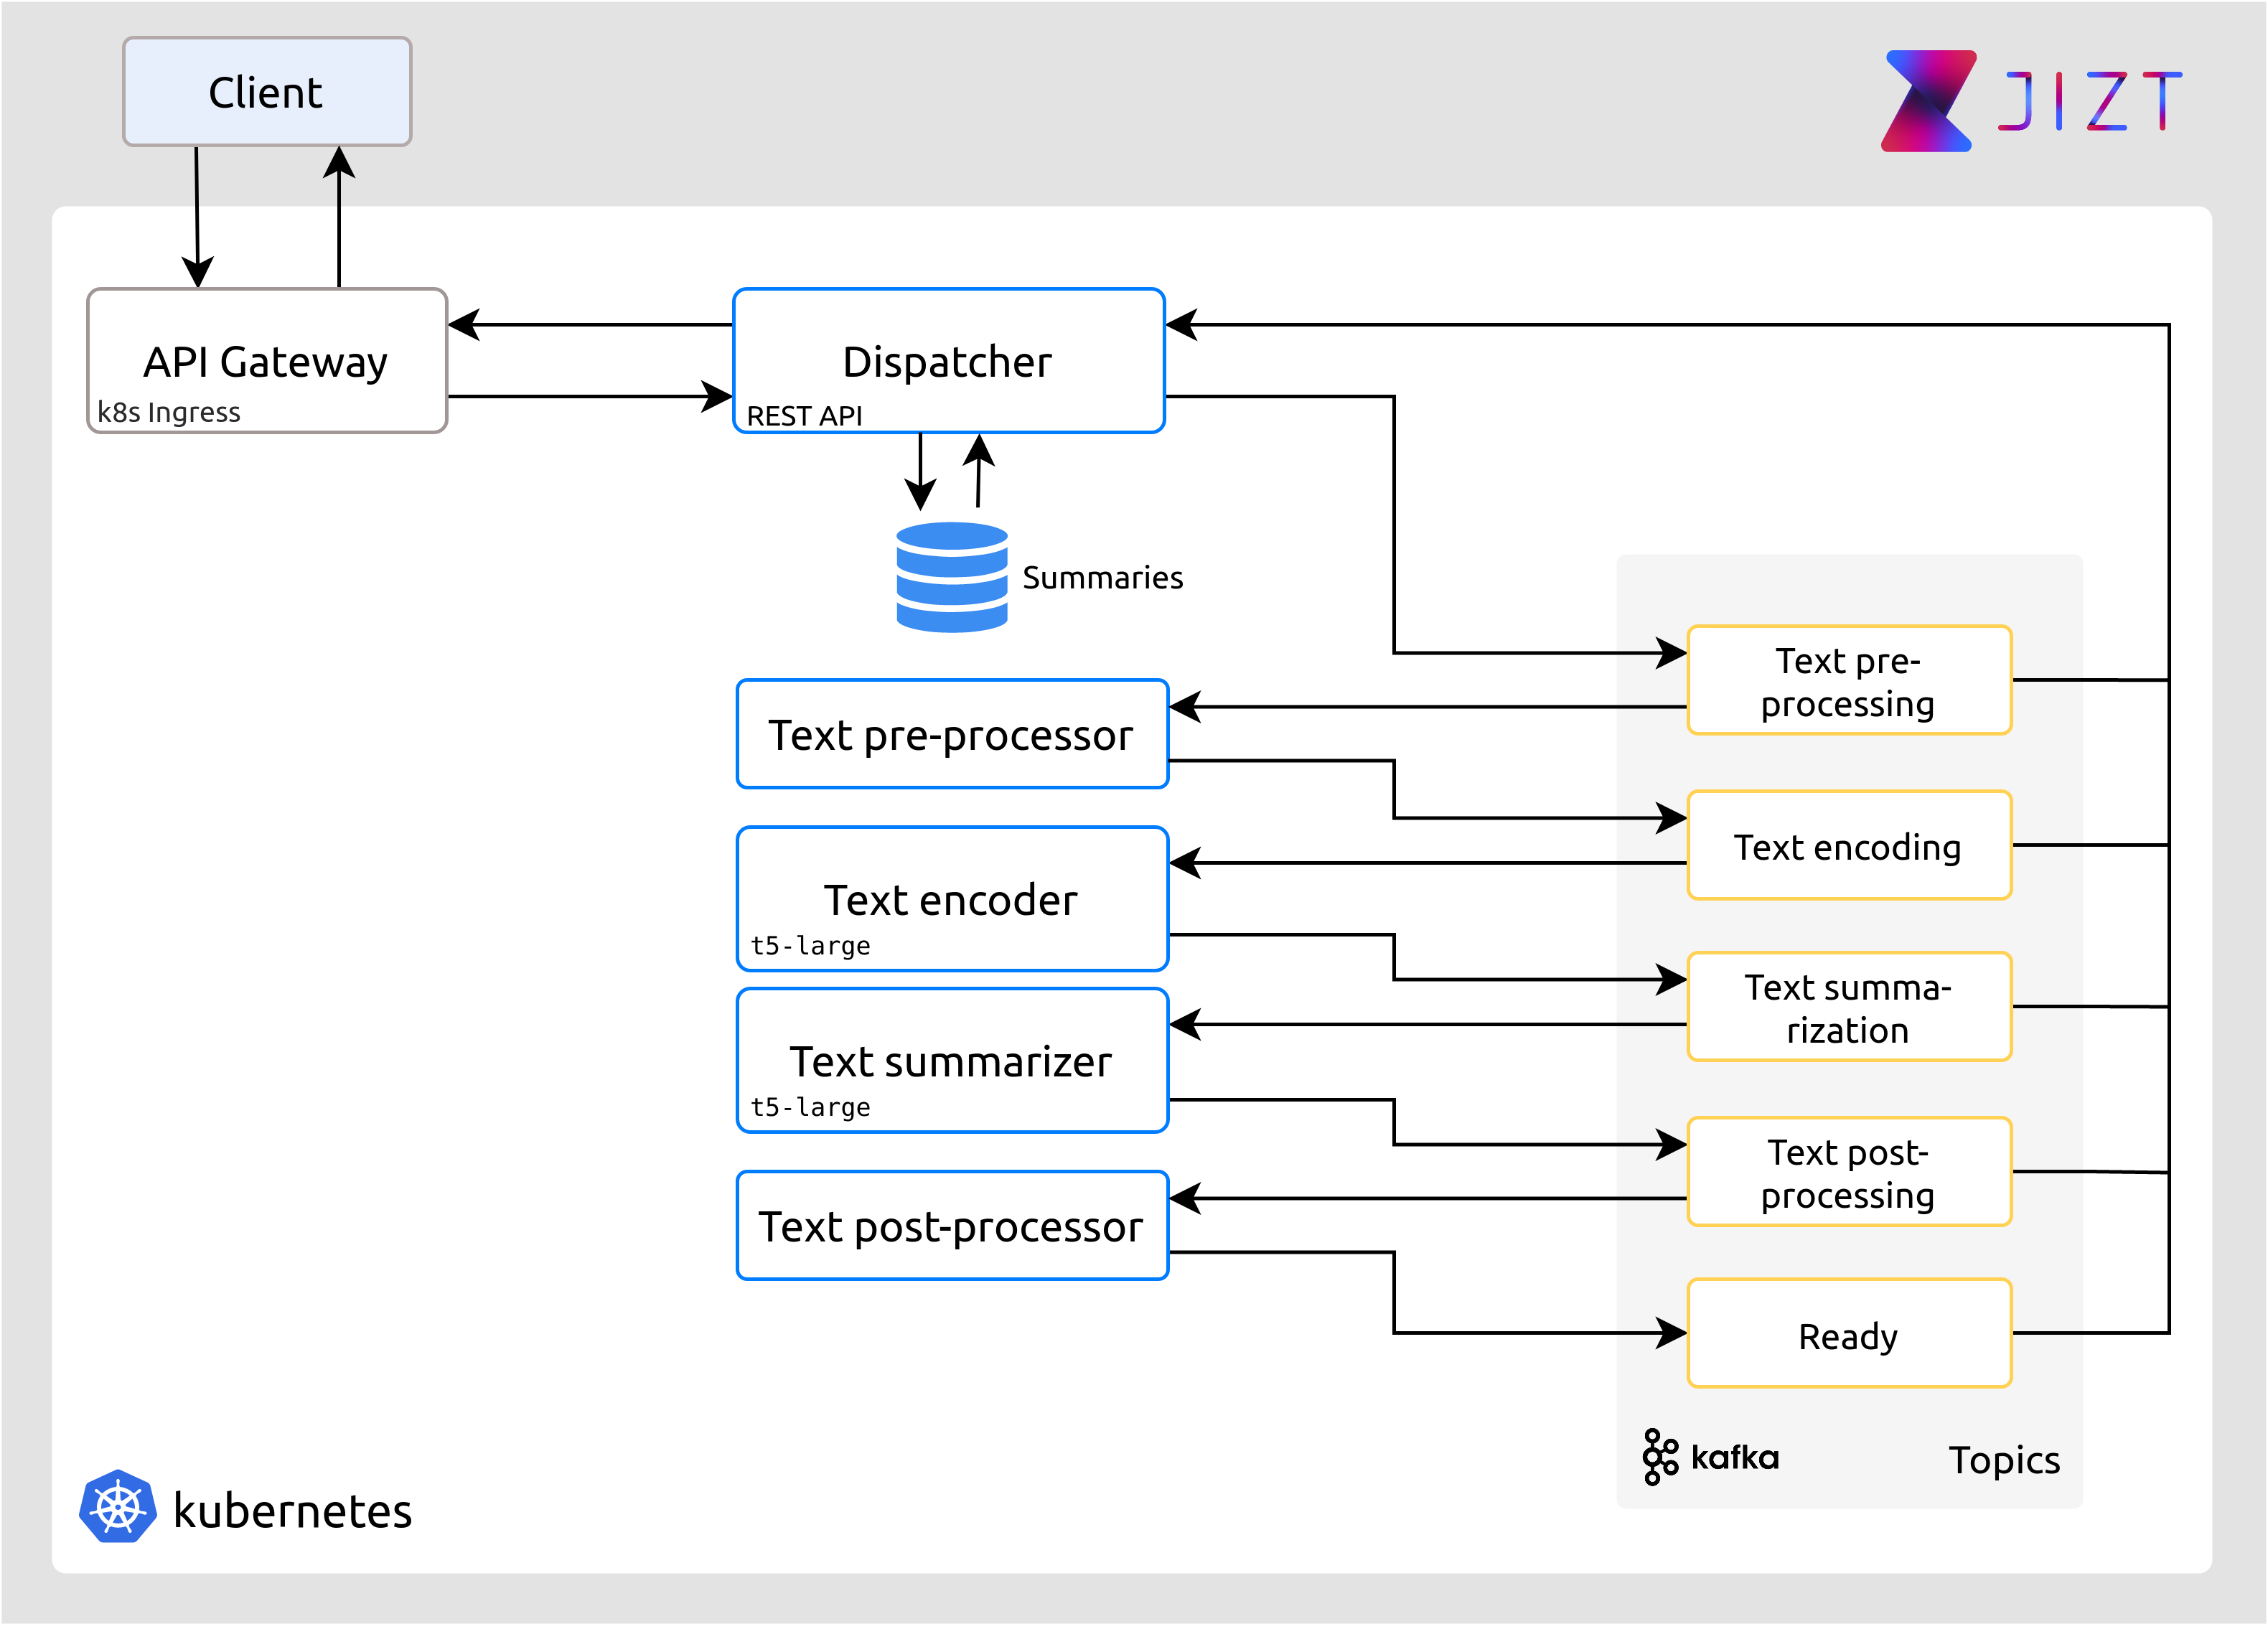
\includegraphics[width=\textwidth]{overview-arch}
	\caption{Vista general de la arquitectura del \emph{backend}.}
	\label{fig:overview-arch-2}
\end{figure}

Con esta figura en mente, el proceso completo que se sigue es el siguiente:

\begin{enumerate}
	\item El cliente realiza una petición HTTP, incluyendo en el cuerpo el texto a resumir, así como los parámetros del resumen a generar.
	
	\item Ingress (API \emph{Gateway}) comprueba que dicha petición se está haciendo a un \emph{endpoint} válido, y en ese caso la redirige hacia el \emph{Dispatcher}.
	
	\item El \emph{Dispatcher} realiza una serie de comprobaciones:
	\begin{enumerate}
		\item Si la petición no contiene ningún texto, se devuelve un error. En el caso de los parámetros, si son incorrectos o inexistentes, se ignoran y se utilizan valores por defecto.
		
		\item Se consulta en la base de datos si ya existe un resumen generado para ese texto con esos parámetros. En ese caso, lo devuelve directamente, sin generar de nuevo el resumen.
		
		\item En caso contrario, produce un mensaje al \emph{topic} del pre-procesador de textos, conteniendo el texto y los parámetros del resumen.
	\end{enumerate}

	\item El pre-procesador está constantemente comprobando si existen mensajes nuevos en su \emph{topic}. En ese caso los consume, realiza las tareas de pre-procesado, y produce el resultado en el \emph{topic} del codificador.
	
	\item Este proceso continua de forma análoga hasta llegar al post-procesador, el cual produce el resumen final al \emph{topic} <<Listo>> (\emph{Ready}). El \emph{Dispatcher}, en ese momento, consume el mensaje, actualiza la base de datos, y proporciona el resumen al cliente.
\end{enumerate}

En dicha \hyperref[fig:overview-arch-2]{figura}, vemos también que el \emph{Dispatcher} consume de todos los \emph{topics}. Esto permite actualizar el \emph{estado} del resumen (pre-procesando, resumiendo, post-procesando, o listo), según va pasando por las diferentes etapas, a fin de proporcionar una retroalimentación más detallada al usuario\footnote{\, Por ahora, el \emph{Dispatcher} solo muestra el estado <<resumiendo>>. El resto de estados se implementarán en futuras iteraciones.}.


\subsection{Helm}

Helm se define frecuentemente como un gestor de paquetes para Kubernetes, aunque en la práctica va más allá.

La configuración de Kubernetes se lleva a cabo, principalmente, de forma declarativa a través de ficheros en formato \texttt{yaml}, lo que en inglés se conoce como \emph{templating}. Nuestro proyecto, el cual es relativamente pequeño, hace uso de más de 20 de estos ficheros de configuración. Es fácil imaginarse, por tanto, que un proyecto de mediana escala contendrá cientos de \emph{templates}.

Helm permite, a través de un único comando, desplegar todos estos componentes de forma automática, gestionando aspectos como el orden en el que se crean los componentes, el cual en muchos casos no es trivial. Una vez instalados, a través de otro comando, podemos actualizar los posibles cambios que haya sufrido alguno de los \emph{templates}, de forma que solo afecte a los componentes involucrados en dichas modificaciones, y sin tiempos de interrupción.

Además, a tráves de las llamadas \emph{Library Charts} \cite{helm-lib-charts}, Helm nos permite generar una plantilla que varios componentes pueden reutilizar. Esto es muy apropiado en nuestro caso dado que todos nuestros microservicios tienen una estructura similar; lo único que cambia es la imagen (contenedor) que implementan.

Una última ventaja es que podemos distribuir el \emph{backend} de JIZT como un único paquete, facilitando su instalación por parte de otros desarrolladores.


\subsection{Crunchy PostgreSQL Operator}

De igual modo que Strimzi facilita el despliegue de Kafka en Kubernetes, el operador para PostgreSQL de Crunchy automatiza y simplifica el despliegue de \emph{clústers} PostgreSQL en Kubernetes. Podemos hablar, por tanto, de <<PostgreSQL como servicio>> \cite{crunchy21}.

De este modo, podemos implementar una base de datos que almacene los resúmenes generados\footnote{\, Una de las futuras historias de usuario implementará un <<modo privado>>, de forma que los usuarios tengan la posibilidad de generar sus resúmenes sin que se almacenen de manera permanente.}, con dos propósitos principales: (a) servir como capa de caché, evitando tener que producir el mismo resumen en repetidas ocasiones, y (b) construir un \emph{dataset} que se podría utilizar en un futuro para tareas de evaluación, o incluso para el entrenamiento de otros modelos.

Este operador coordina de forma automática los accesos a la base de datos, asegurando la integridad de la misma. Esto es posible dado que solo existe un única instancia (\emph{pod}) con capacidades de escritura-lectura. El resto de instancias que accedan a la base de datos, solo podrán leer de la misma. Si la instancia primaria fallara, el operador se encargaría inmediatamente de elegir otra instancia como primaria.


\subsection{Docker}

Docker nos permite encapsular nuestros microservicios en contenedores. De este modo, gracias a Kubernetes, podemos crear réplicas de cada microservicio, haciendo posible el escalado de nuestro sistema.

A diferencia de las máquinas virtuales, en las cuales el sistema operativo subyacente se comparte a través del hipervisor, cada contenedor Docker ejecuta su propio sistema operativo, como podemos ver en la \hyperref[fig:vm-container]{siguiente figura}:

\begin{figure}[!h]
	\centering
	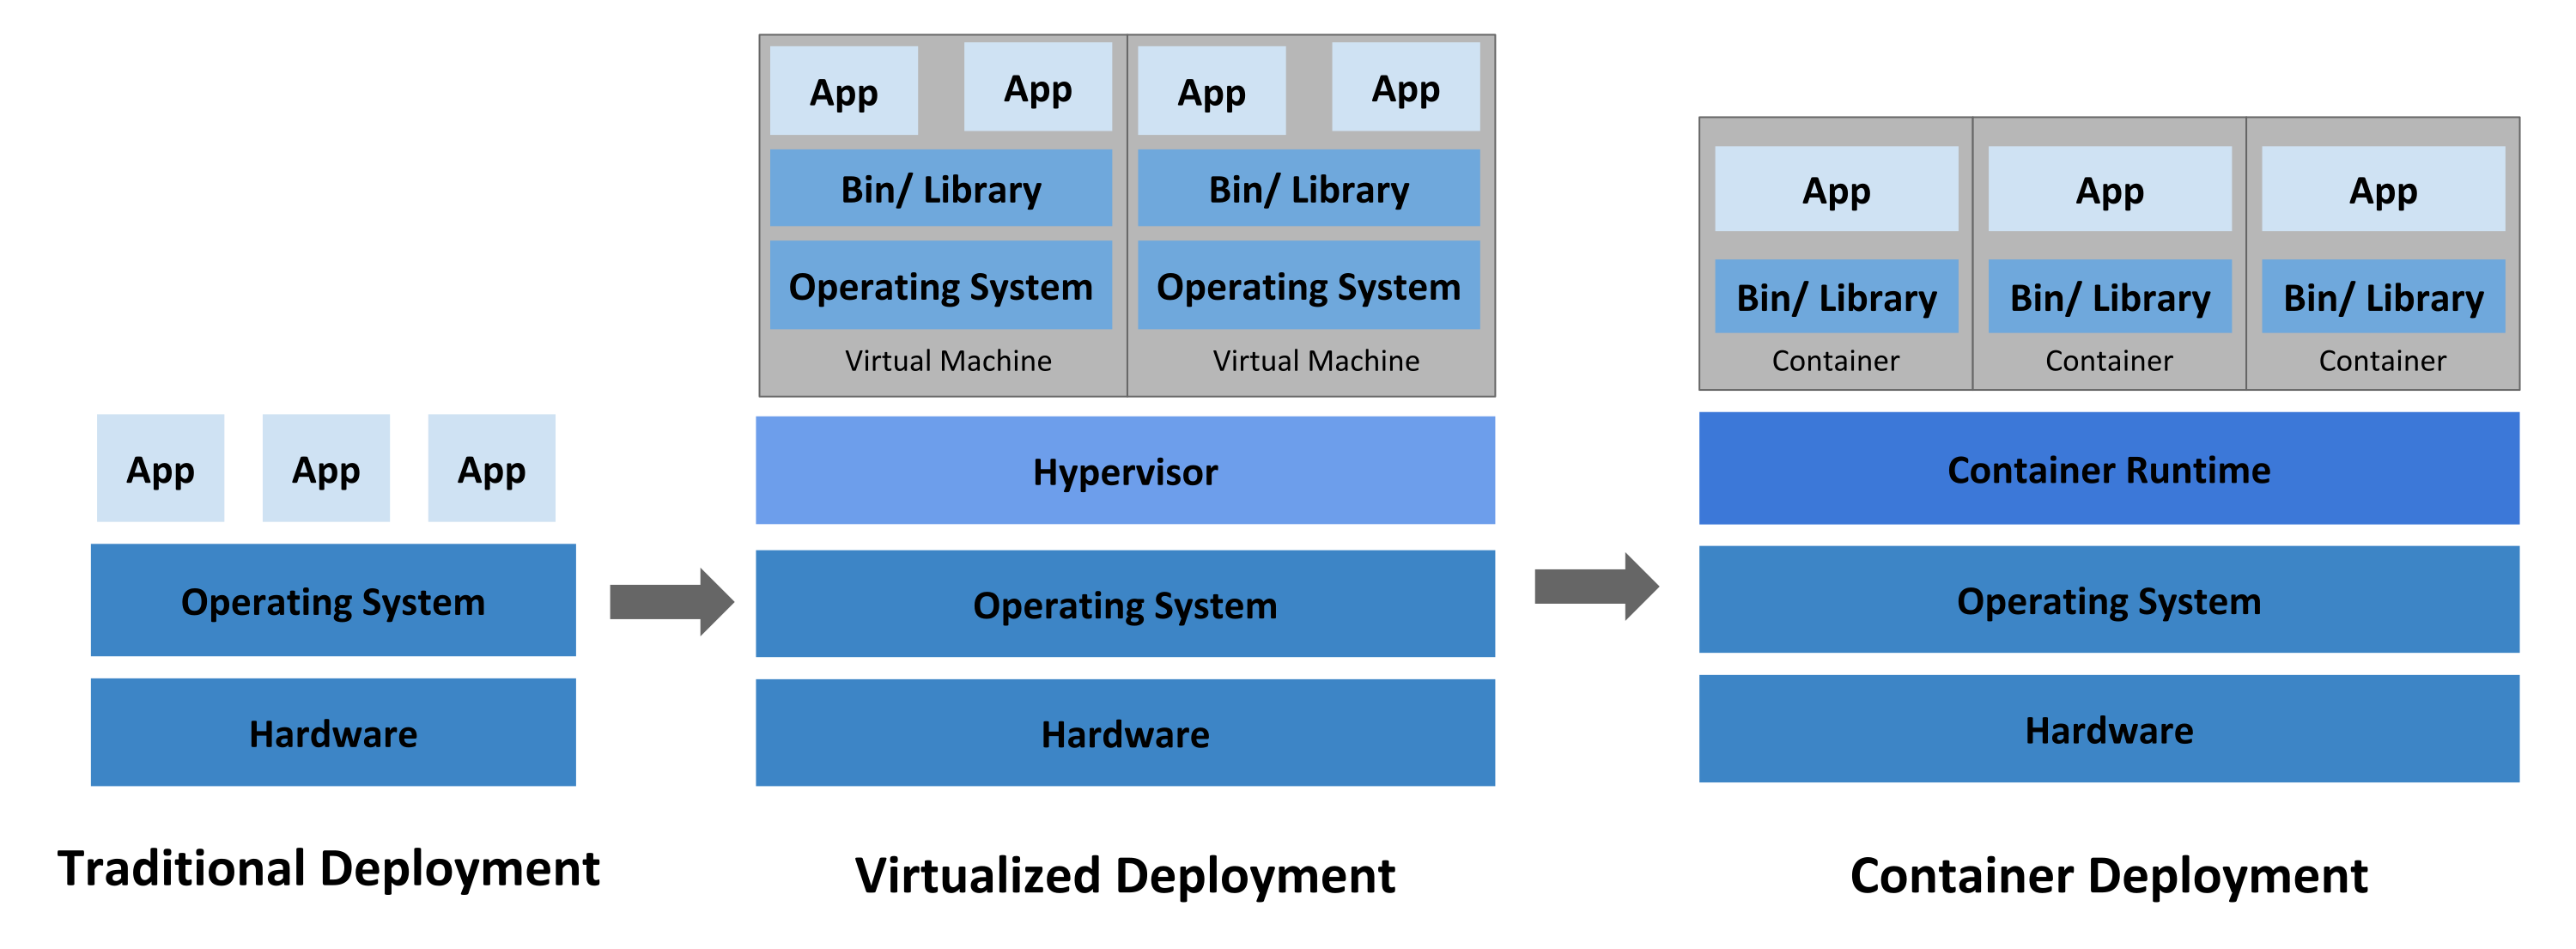
\includegraphics[width=\textwidth]{docker}
	\caption[Diferentes enfoques en el despliegue de sistemas \cite{kubernetes}.]{Comparativa de los diferentes enfoques en el despliegue de sistemas \cite{kubernetes}.}
	\label{fig:vm-container}
\end{figure}

Otra ventaja de Docker es que nos permite distribuir la implementación de nuestros microservicios a través imágenes, por lo que un desarrollador que solo quisiera hacer uso de uno de los microservicios, podría hacerlo de manera sencilla.


\subsection{Flask y Flask-RESTful}

Flask es uno de los \emph{frameworks} más populares para la creación de aplicaciones \emph{web} en Python\cite{flask}, concebido para ser lo más simple posible. En nuestro caso, hemos empleado esta herramienta para implementar la lógica de la API REST. Además, hemos utilizado una conocida extensión de Flask, Flask-RESTful \cite{flaskRestful}, orientada a la construcción de APIs REST, como es nuestro caso.

Dado que es el \emph{Dispatcher} quien implementa la REST API, es únicamente este microservicio el que hace uso de este \emph{framework}.


\section{\emph{Frontend}} \label{sec:frontend}

\subsection{Flutter}

Flutter un \emph{kit} de herramientas de UI (interfaz de usuario) que, a partir del mismo código fuente base, permite compilar de forma nativa aplicaciones para móvil, \emph{web} y escritorio \cite{flutter-es}, lo cual permite \cite{miola20}:

\vspace{-0.5cm}
\begin{itemize}
	\item [\textbullet] Un desarrollo más rápido, dado que solo se trabaja en una única base de código.
	\item [\textbullet] Costes más bajos, ya que solo mantenemos un proyecto en vez de varios.
	\item [\textbullet] Una mayor consistencia, proporcionando al usuario la misma interfaz gráfica y herramientas en las distintas plataformas.
\end{itemize}

Pese a ser desarrollado por Google desde su nacimiento en 2017, Flutter cuenta en la actualidad con un gran apoyo de la comunidad \emph{open-source}. Esto ha facilitado la resolución de dudas y errores a la hora de desarrollar nuestra aplicación.

Flutter emplea el lenguaje Dart, el cual guarda similitudes con otros lenguajes como Java o C\#. Existen numerosos aspectos de Flutter y Dart que cabría explicar; no obstante, en pos de la brevedad introduciremos uno de los que más interesantes y relevantes nos parecen para este proyecto: ¿Cómo se consigue que Dart pueda ser ejecutado nativamente en plataformas que pueden resultar tan dispares como Android, iOS, \emph{web}, Windows o Linux?

Para responder a esta pregunta, veamos una a una las opciones que ofrece Dart a la hora de ser compilado ejecutado.

\subsubsection{Ejecución independiente (\emph{stand-alone})}

Esta opción es similar a cómo otros lenguajes, como Java, trabajan. Así como Java requiere de la JVM (\emph{Java Virtual Machine}) para ejecutarse, Dart también dispone de su DVM (\emph{Dart Virtual Machine}).

No obstante, utilizando Dart de este modo, solo podremos ejecutarlo si existe una DVM. Para poderlo ejecutar en cualquier plataforma, necesitamos usarlo en conjunción con Flutter \cite{miola20}.


\subsubsection{Compilación anticipada (AOT, \emph{Ahead-of-time} Compilation)}

La compilación AOT consiste en traducir un lenguaje de alto nivel, como en este caso Dart, en código máquina nativo \cite{aot-wiki}. Este código máquina sí que será dependiente del sistema.

Gracias a la compilación anticipada, podemos obtener, a partir de nuestro código escrito en Dart, un fichero ejecutable para las distintas plataformas, esto es \texttt{.apk} o \texttt{.aab} para Android, \texttt{.exe} para Windows, etc..


\subsubsection{\emph{Web}}

El código Dart también puede ser traducido a HTML, CSS y JavaScript. Esto significa que podemos ejecutar nuestra aplicación en Chrome o Firefox\footnote{Por ahora, solo Chrome, Safari, Edge y Firefox están soportados, este último solo en su versión de escritorio con WebGL habilitado.}, y la interfaz gráfica será la misma que en el resto de plataformas.

Es importante mencionar, que el soporte para \emph{web} de Flutter se encuentra aún en fase \emph{beta}, por lo que no se recomienda para producción \cite{flutter-web}.

No obstante, nosotros no hemos experimentado problemas con nuestra aplicación en ninguno de los navegadores soportados.